\section{Introduction}

% TODO: Review the list below
This chapter describes implementation details of different components of the project. All of these components are part of the AcousticBrainz Server\footnote{\url{https://github.com/metabrainz/acousticbrainz-server}}:
\begin{itemize}
    \item Dataset creation
    \item Model training
    \item Challenge management interface
    \item Dataset submission process and different stages of a challenge
    \item Evaluation of results
\end{itemize}

%%%%%%

\section{Dataset creation}

\subsection{Overview}

To cover most basic use cases we have three ways to create a dataset:
\begin{itemize}
    \item Web-based editor
    \item Importer from CSV file
    \item Web API
\end{itemize}

The overview of how datasets are processed and used in the projects is shown in figure \ref{fig:dataset_creation}.

\begin{figure}[h]
  \centering
  \includegraphics[width=0.80\textwidth]{dataset_creation}
    \caption{Overview of the dataset lifetime in the AcousticBrainz project}
    \label{fig:dataset_creation}
\end{figure}

\subsection{Web-based editor}

The easiest way for people to start building a dataset is to use an editor that is integrated with the AcousticBrainz website. It doesn't require user to have any additional tools.

Editor interface is implemented using a JavaScript framework called ``React''\footnote{\url{https://facebook.github.io/react/}}. It allowed us to build an interface that is easy and fast to use. Behind the scenes, it relies on the web API of AcousticBrainz Server which provides endpoints for editing datasets. Same API can be used by people to create datasets directly using their own tools. We think it's a good idea to use the same interface that is available to the rest of users. That way we can make sure that it is as complete as possible. It is also a good software engineering practice to have a multitier architecture\footnote{\url{https://en.wikipedia.org/wiki/Multitier_architecture}}.

\begin{figure}[h]
  \centering
  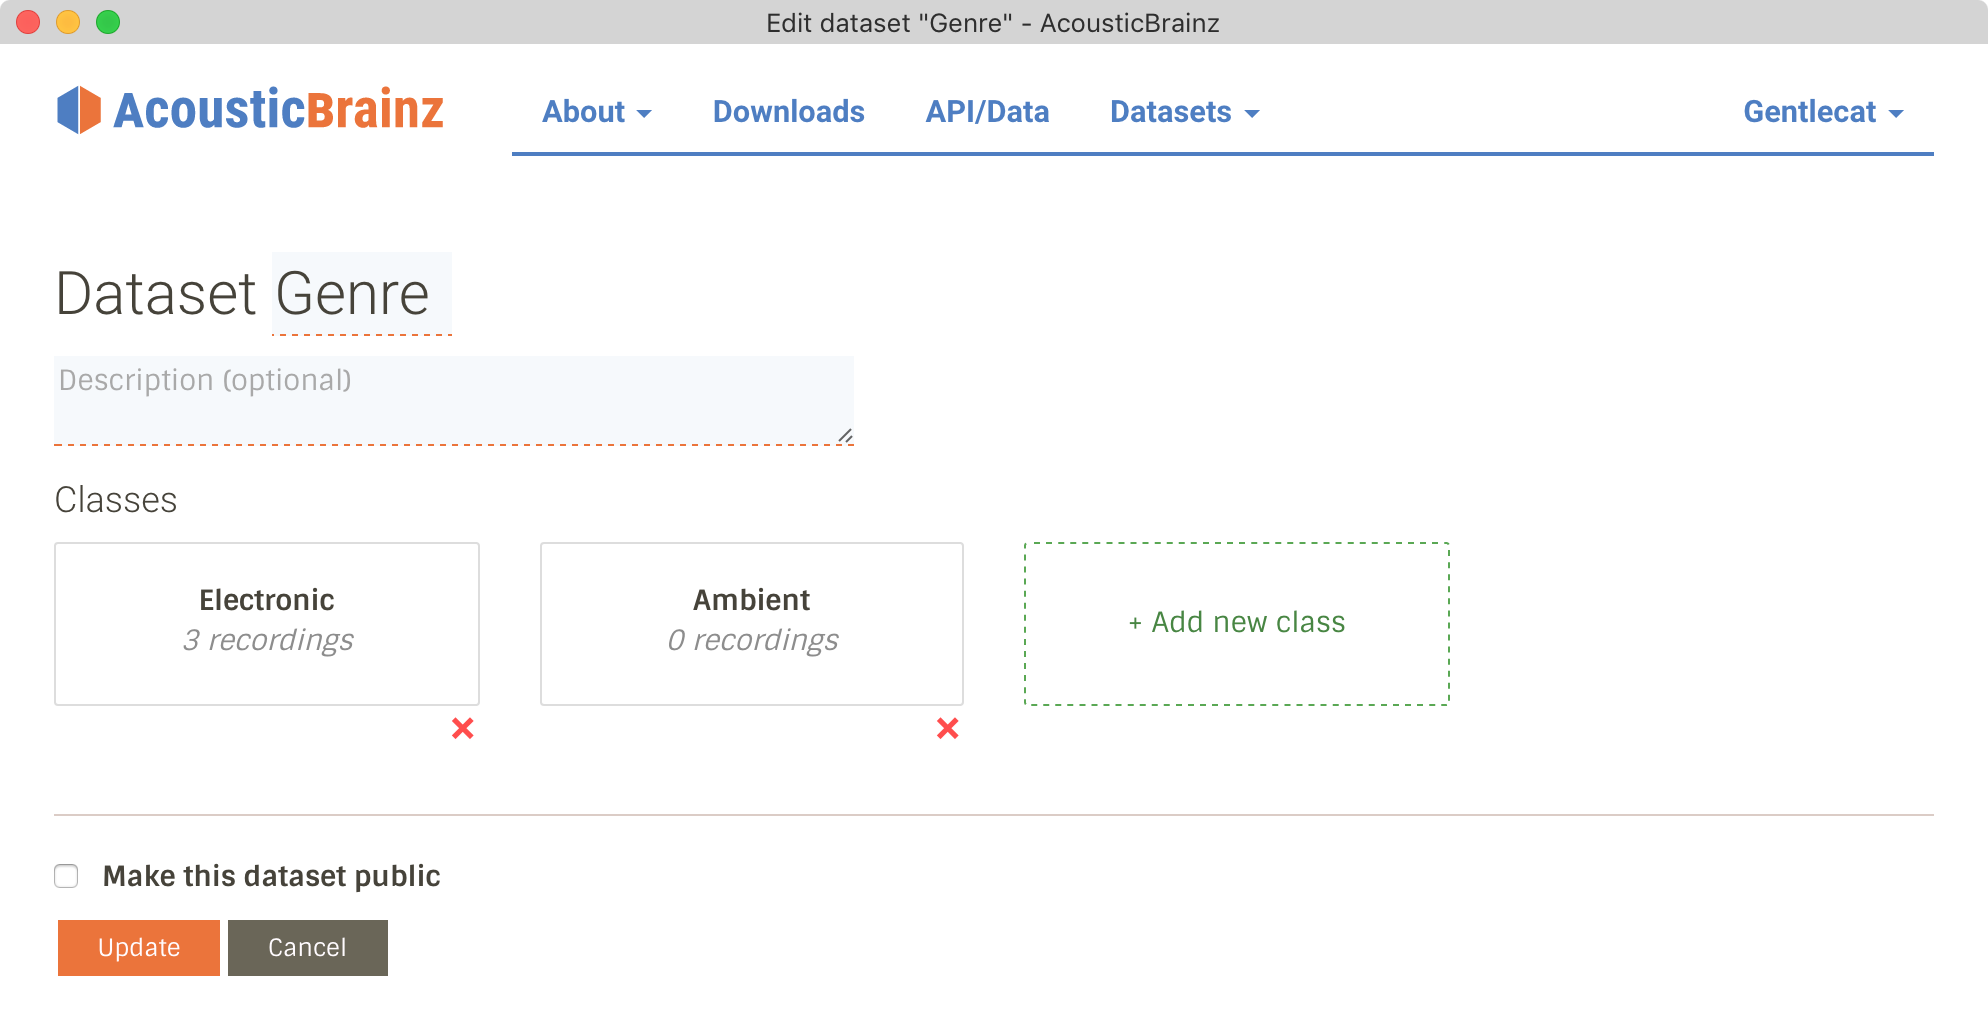
\includegraphics[width=\textwidth]{editor_overview}
    \caption{Main page of the dataset editor}
    \label{fig:editor_overview}
\end{figure}

Figure \ref{fig:dataset_creation} shows the main view of the dataset editor. Here user can do the most basic things like naming a dataset, describing it, defining its structure by specifying a set of classes. From that view users can access each individual class.

\begin{figure}[h]
  \centering
  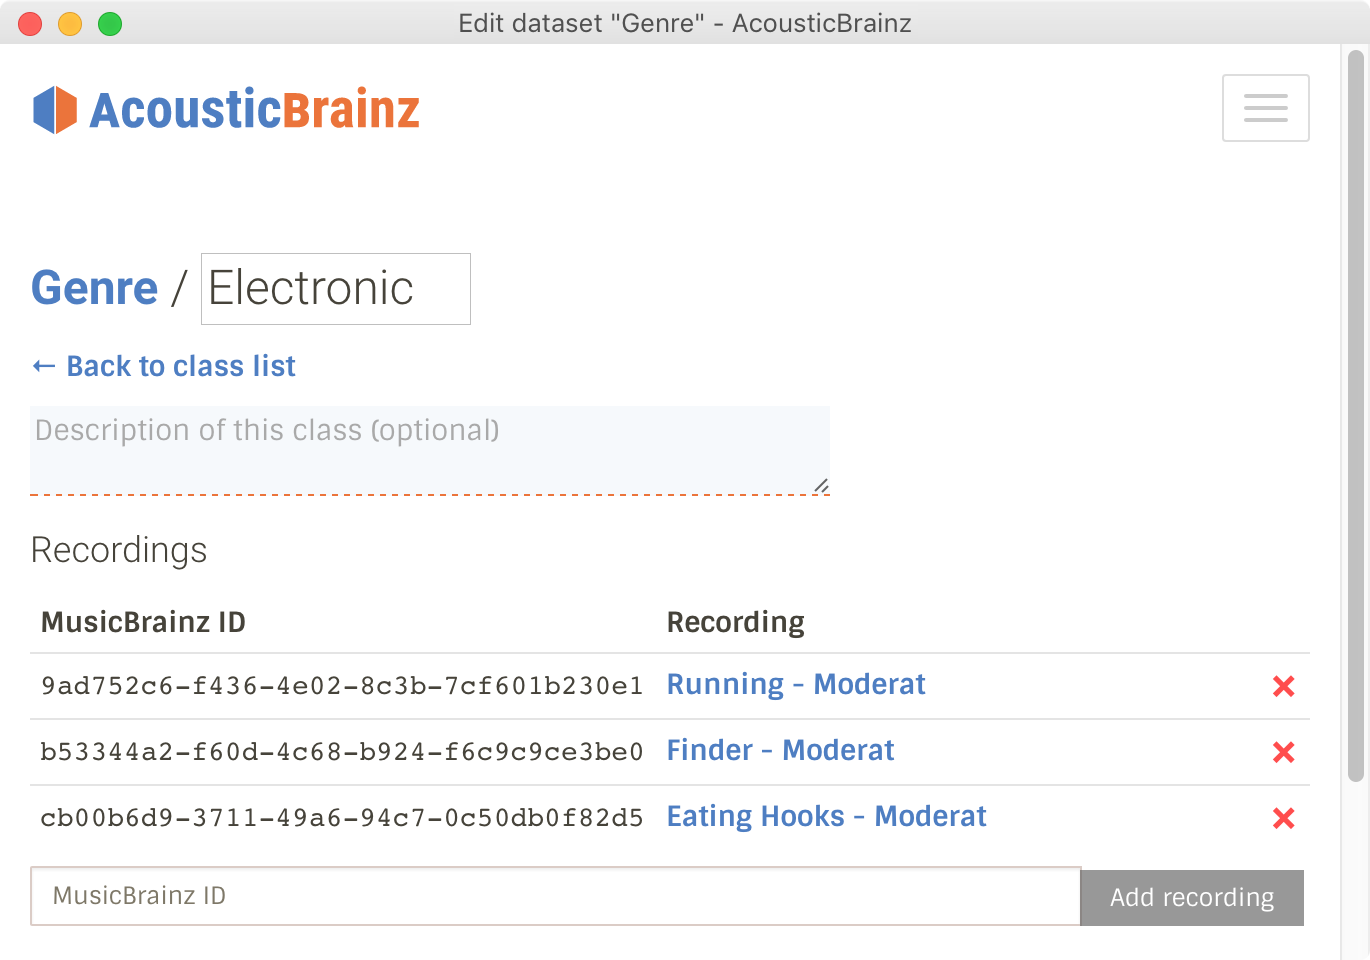
\includegraphics[width=\textwidth]{editor_class}
    \caption{Class view in the dataset editor}
    \label{fig:editor_class}
\end{figure}

In the class view (figure \ref{fig:editor_class}) it's possible to modify recordings\footnote{\url{https://musicbrainz.org/doc/Recording}} that each class contains. All recordings are referenced by MBIDs. For each recording we load its name and name of the associated artist(s) from the MusicBrainz Web Service.

When user is done editing a dataset they can save the changes.

\subsection{CSV importing}

Some researches have their own tools that they work with and, specifically, build and analyze datasets: MATLAB, Python, etc. We think that it would be useful to add a simple way for the to get started using new features in AcousitcBrainz project by importing their datasets in CSV format\footnote{\url{https://tools.ietf.org/html/rfc4180}}.

Supported CSV files must have the following structure: \textit{\textless MusicBrainz Identifier of a recording\textgreater, \textless Class label\textgreater}. Each row in the file defines an ID of a recording and associated class label. After CSV file is ready for import, it can be uploaded to AcousticBrainz where it will be parsed, converted and stored for further use.

\subsection{Web API}

The last way of working with datasets we have is using a web API\footnote{Application Programming Interface, \url{https://en.wikipedia.org/wiki/Web_API}}. It allows users to create and edit datasets by sending HTTP\footnote{\url{http://httpwg.org/specs/}} requests to AcousticBrainz server.

API has the following endpoints:
\begin{itemize}
    \item Create a dataset
    \item Retrieve a dataset
    \item Update details (name, description) of a dataset
    \item Delete a dataset
    \item Add class to a dataset
    \item Update class in a dataset (name, description)
    \item Remove class from a dataset
    \item Add recordings into a class
    \item Remove recordings from a class
\end{itemize}

\textit{All of these endpoints are described in more detail in AcousticBrainz documentation\footnote{\url{https://acousticbrainz.readthedocs.io/api.html\#datasets}}.} It is a useful addition to existing ways to create a dataset, which can encourage users to make their own tools that can help with the creation process.

\subsubsection{Authentication}

Authentication is done using API keys that need to be passed with every request. In order to obtain an API key, users need to login into their AcousticBrainz profile and click ``Generate new key'' button (see figure \ref{fig:api_key}).

\begin{figure}[h]
  \centering
  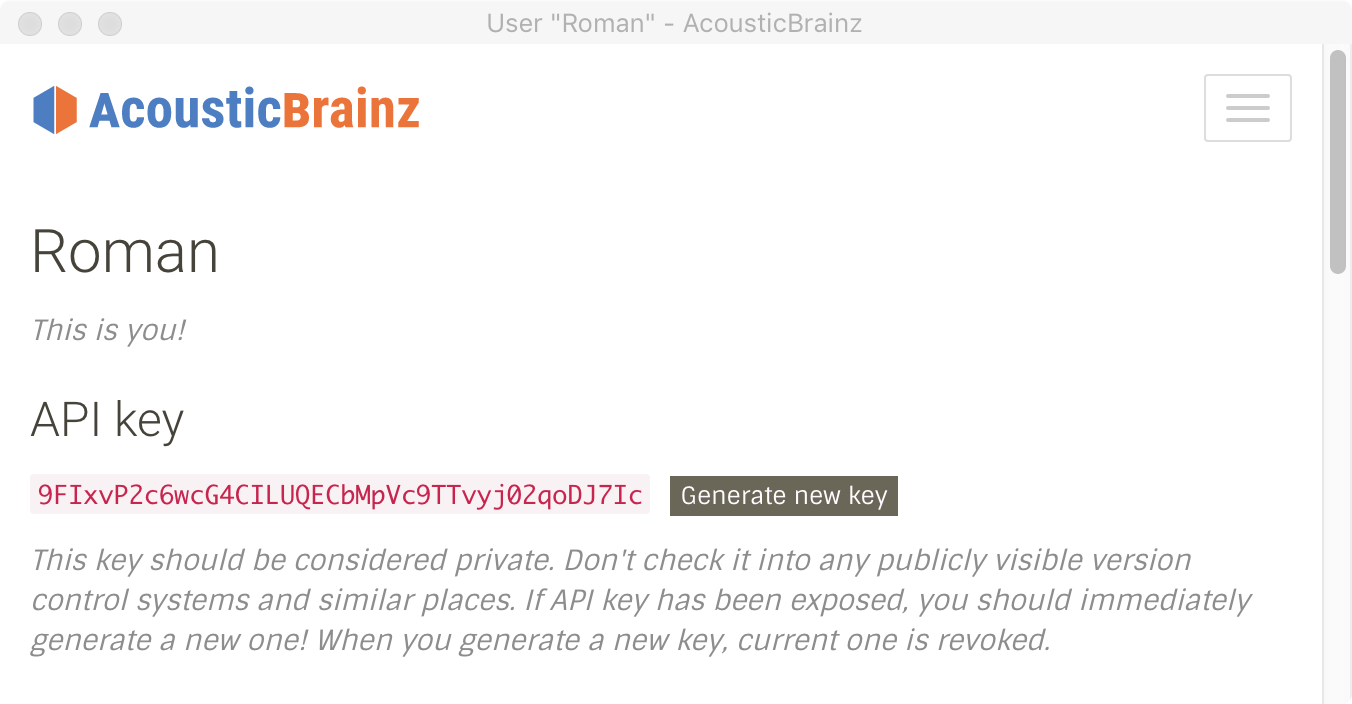
\includegraphics[width=0.80\textwidth]{api_key}
    \caption{Profile page with API key generator}
    \label{fig:api_key}
\end{figure}

API key is randomly generated from lowercase and uppercase ASCII\footnote{American Standard Code for Information Interchange, \url{https://en.wikipedia.org/wiki/ASCII}} letters and digits. Its length is always 40 characters. Currently, only one API key per user account is allowed.

All keys are meant to be kept private. Person who has access to a specific API key can perform actions on behalf on the owner of that key. In case the key is exposed, it is possible (and highly recommended) to generate a new one.

The key privacy limitation means that some uses can become more complicated. For example, in order to build a web application on top of AcousticBrainz API there will need to be a back-end server that would store the API key and attach it to all requests to AcousticBrainz. This, however, shouldn't be a factor when only one person is using a key.

\cite{farrell2009api} describes how API keys are typically used with web APIs, some of the issues involved, and ways to improve. He recommends to use OAuth protocol\footnote{\url{http://oauth.net/}} as a better alternative. This can be one of the future improvements that we make in AcousticBrainz.

%%%%%%

\section{Challenges}

\subsection{Challenge lifetime}

From start to finish each challenge is composed of the following steps:
\begin{enumerate}
    \item Organizer creates a challenge.
    \item Challenge begins and participants submit their datasets.
    \item Submission period ends.
    \item Challenge concludes after results are calculated.
\end{enumerate}

\begin{figure}[h]
  \centering
  \includegraphics[width=\textwidth]{challenge}
    \caption{Overview of the challenge process}
    \label{fig:challenge}
\end{figure}

\subsubsection{Creation of a challenge}

When organizer creates a challenge, they need to define its name, set of classes that are required to be in a dataset, reference to validation dataset that will be used to measure accuracy of submissions, and a time period in which submissions are going to be accepted. After creation, each challenge is assigned a UUID\footnote{Universally Unique IDentifier, \url{https://tools.ietf.org/html/rfc4122}}, which is used to reference it throughout the project.

Set of required classes is used to define a ``namespace'' that all submissions must follow. All of the classes must be present in a submission, additional classes aren't allowed. Same requirements apply to the validation dataset, which is checked during creation.

Interface for creating (see figure \ref{fig:create_challenge}) a challenge is currently available only in the ``admin'' interface, which is accessible to several trusted users. In the future, if needed, challenge creation tools could be made available to all users of AcousticBrainz project.

\begin{figure}[h]
  \centering
  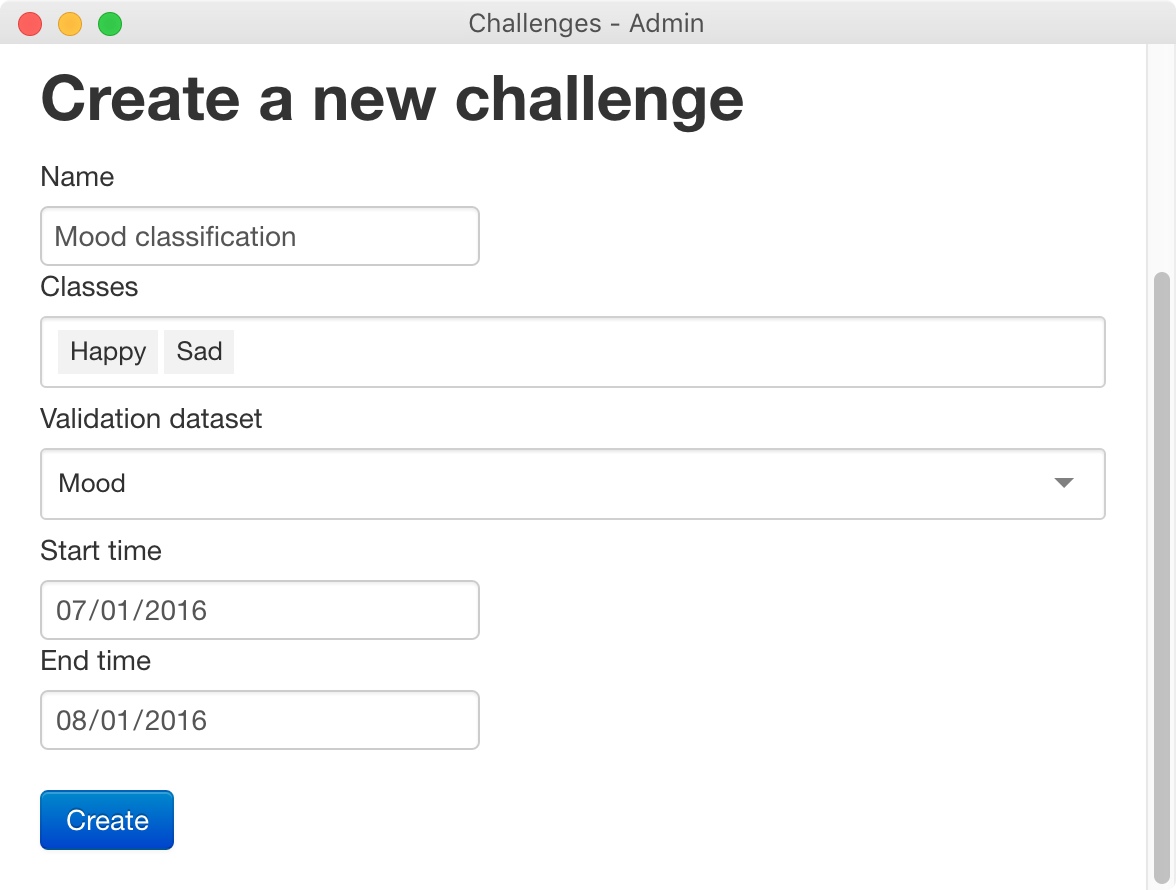
\includegraphics[width=0.80\textwidth]{create_challenge}
    \caption{Challenge creation interface}
    \label{fig:create_challenge}
\end{figure}

\subsubsection{Accepting submissions}

Participation in challenges is open to every user of AcousticBrainz. After creating a dataset with required structure using existing tools, they can submit it for model training as a part of a challenge.

\begin{figure}[h]
  \centering
  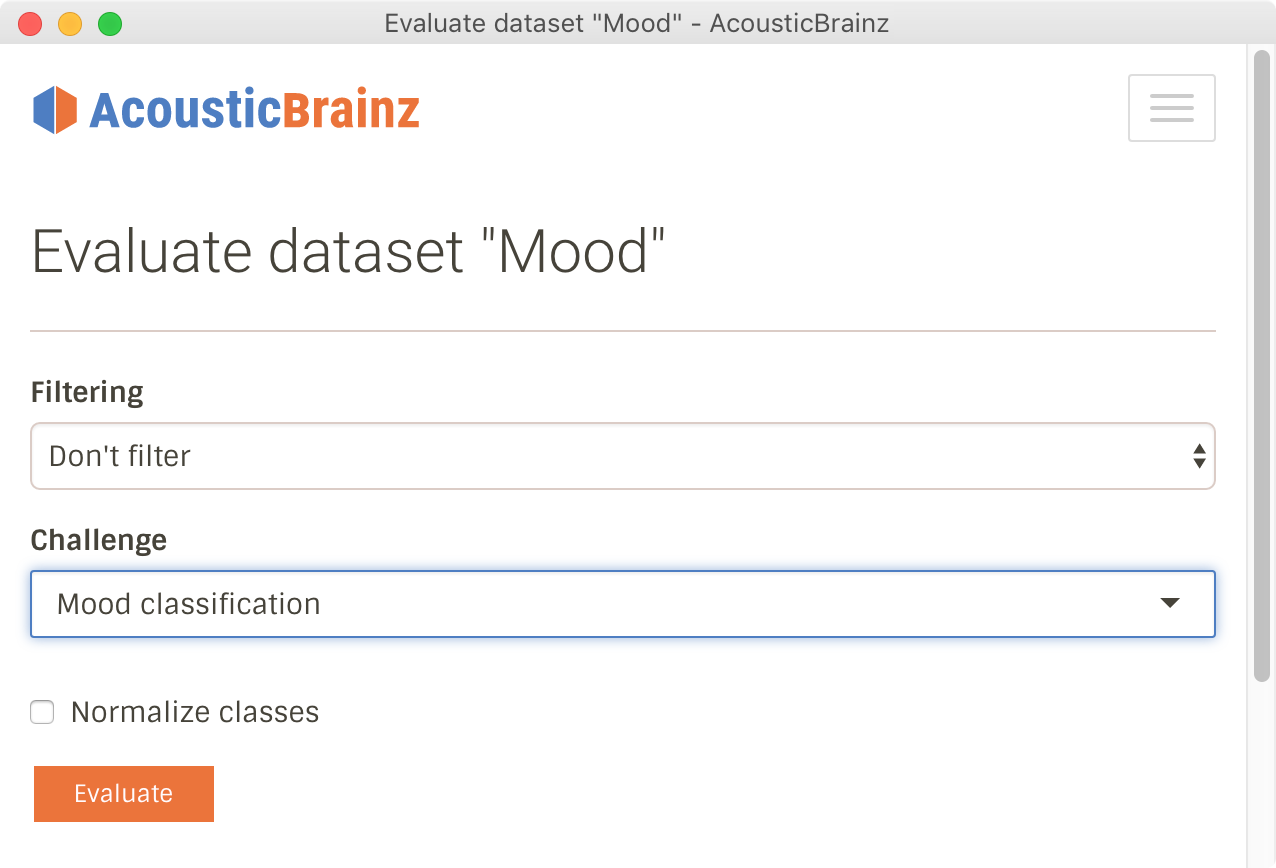
\includegraphics[width=0.80\textwidth]{eval_submission}
    \caption{Training submission interface}
    \label{fig:eval_submission}
\end{figure}

When dataset is submitted, new model training job is added into the queue. In addition to that, dataset structure (list of classes) is checked to make sure that it matches requirements of a challenge. Recording filtering is applied to it (described further).

\subsubsection{Snapshots of datasets}

When user adds dataset into the training queue, regardless of whether it is submitted for a challenge or not, a new snapshot is created. Snapshot of a dataset captures its exact structure at a point of creation: all classes and recordings in them. Snapshots are used to ensure that dataset submitted for model training has a fixed state while it's waiting in the queue or after model is trained. This helps ensure that results (high-level models) are reproducible.

All snapshots are public by default unless they are a part of an ongoing challenge. Snapshots of datasets that are submitted for a challenge need to be private to make sure that other participants can't copy a dataset and make slight modifications that would be enough to increase the accuracy. After challenge concludes, all the snapshots of datasets submitted for it are made available to the public. Participants can compare their datasets, combine them together, and do any other improvements.

In addition to hiding snapshots, users are advised to keep datasets that they are going to submit for a challenge private until it concludes. This is done in a form of a warning during the submission process.

\subsubsection{Evaluating submissions}

There are two stages in evaluation of datasets submitted for a challenge:
\begin{enumerate}
    \item Generation of a model from a dataset.
    \item Measuring accuracy of a model using the validation dataset.
\end{enumerate}

First stage is performed by existing model training script that uses Gaia library\footnote{\url{https://github.com/MTG/gaia}}. That script goes through all datasets submitted for training, generates a model file and performance statistics for each of them.

Second stage is specific to training of datasets submitted for a challenge. In order to ensure that all submissions can be compared fairly, we need to use a separate validation dataset. After original script generates a model, it is used to calculate high-level classes for all items in validation dataset associated with a challenge.

The challenge doesn't conclude until accuracy of all models, generated as a part of it, is measured using validation dataset. When accuracy calculation is done for all submissions, this script marks challenge as concluded. Then overall results can then be viewed on the website.

\subsection{Validation dataset}

Validation dataset is associated with a challenge during challenge creation step. This dataset is built using the usual tools (web UI, API, or CSV importer) by organizer of a challenge.

It is important to have this dataset to be able to fairly compare submissions for a challenge. Measurement is done on a model generated from submitted dataset.

\subsubsection{Availability and filtering}

Validation dataset is made public to help challenge participants remove doubt about the structure, which can happen in case it is hidden and there is no way to inspect a set of recordings that is used to measure submissions. Participants might doubt that quality of this dataset is any good and the accuracy measurements that are based on it are correct.

Having a validation dataset public means that filtering becomes mandatory. Dataset submitted for a challenge can't contain the same recordings as validation dataset when it goes into the model training. There are two main types of filtering we can have:
\begin{itemize}
    \item Recording filtering
    \item Artist filtering
\end{itemize}
One thing that needs to be kept in mind when choosing type of filtering is that some of them might be unsuited for some classification task. For example, when creating a challenge for classifying an artist, artist filtering cannot be used.

%%%%%%

\section{User feedback}

User feedback is a useful tool for understanding how models perform in real world conditions and improving existing datasets. It can be submitted for all high-level data computed from models that are applied to all data in AcousticBrainz.

Users submit feedback using ``Correct'' or ``Incorrect'' buttons. If users think that result of classification is \emph{incorrect} they can also specify what result is expected. Expected result must be one of the classes from a dataset (its snapshot) that the model is based on. When users send their feedback, it's stored in a database for further use.

%%%%%%

\section{Source code}

As was said in the introduction, one of the main goals of the project is to be as open as possible. All the source code for the work that has been done for this project and before it is available to everyone under an open source licence (GNU General Public License, version 2). It is located in a Git\footnote{\url{https://git-scm.com/}} repository at \url{https://github.com/metabrainz/acousticbrainz-server}.

Anyone is free to examine the underlying implementation of the project, its components. Users are encouraged to contribute their improvements or fixes for problems that they encounter while using the project. Alternatively, they can report issues in our issue tracking software (JIRA) at \url{https://tickets.musicbrainz.org/browse/AB}.

All code contributions, including ones that were made within this master's project, undergo code review process that all contributors participate in. This helps us improve code quality and helps keep track of changes that happen over time.
